\documentclass[a4paper,12pt]{article}

\usepackage[french]{babel}   % Active la langue française
\usepackage{graphicx}    	% Pour insérer des images
\usepackage{lipsum}      	% Pour du texte factice
\usepackage{fancyhdr}    	% Pour personnaliser les en-têtes et pieds de page
\usepackage{listings}    	% Pour afficher le code
\usepackage{xcolor}      	% Pour personnaliser les couleurs
\usepackage{minted}      	% Pour une coloration syntaxique avancée
\usepackage{amsmath}     	% Pour les équations
\usepackage{hyperref}    	% Pour les liens cliquables
\usepackage{tcolorbox}
\usepackage{lmodern}


\hypersetup{
	colorlinks=true,   	% Active les liens en couleur
	linkcolor=blue,    	% Couleur des liens internes
	urlcolor=blue,     	% Couleur des liens externes
	citecolor=blue     	% Couleur des liens de citation
}



\pagestyle{fancy}  % Active le style personnalisé
\fancyhf{}  % Efface les en-têtes et pieds de page par défaut


\fancyfoot[R]{
\includegraphics[width=1.3cm]{logo.png}}


% Ajouter la numérotation des pages à droite du pied de page
\fancyfoot[C]{\thepage}

\renewcommand{\sectionmark}[1]{\markboth{#1}{}}

% Afficher la section courante à gauche du pied de page
\fancyfoot[L]{\nouppercase{\leftmark}}

\begin{document}

% ---- Page de titre ----
\begin{titlepage}
	\centering
	
\includegraphics[width=4cm]{logo.png} \\[1cm]  % Ajuste la taille du logo

	{\LARGE \textbf{Etude de la dynamique des foules}} \\[0.5cm]
    
	{\large Par le biais de la physique moderne} \\[1.5cm]

	\textbf{Auteurs :} \\[0.3cm]
	NADAUD Antonin \\
	JANINI  Raphaël \\
	LUBIN Thomas \\
	NUCE LAMOTHE Augustin \\[1cm]

	\textbf{Encadrant :} \\[0.3cm]
	DESPLAT Lucie \\[1.5cm]

	\textbf{\today}  % Affiche la date du jour
	\\[2cm]

	\vfill % Remplit l'espace verticalement pour centrer

	{\large CY Tech – préing-2 groupe 2} \\

\end{titlepage}

% --- page blanche ---
\newpage
\thispagestyle{empty}  % Pas de numérotation, ni d'en-tête/pied de page
\mbox{}  % Crée une page vide (avec un espace vide)

% ---- Sommaire ----
\newpage


\renewcommand{\contentsname}{Sommaire}  % Change "Contents" en "Sommaire"
\thispagestyle{empty}
\tableofcontents  % Génère le sommaire automatiquement avec des liens cliquables

% ---- introduction --- 
\newpage

\setcounter{page}{1} % -- met la page à 1 --

\section{Objectif}
\subsection{Situation 1}
\indent La première situation (imposée) dans le cadre de cette étude, consiste à modéliser l’évacuation d’une foule depuis un espace rectangulaire, tel qu’une salle. Les individus se dirigent vers une sortie sous l'effet d'une force motrice, tout en interagissant les uns avec les autres par le biais de forces sociales. Chaque individu est associé à une vitesse cible, représentant son intention de déplacement. L'objectif est d'avoir le temps d'évacuation totale pour la foulle

\subsection{Situation 2}
\indent On repart sur les bases de la situation une, mais cette fois dans une salle de cour. On ajoute aussi le sentiment de panique pour certains individus, modélisée par une vitesse plus importante. L'objectif est de savoir combien de personne doivent paniquer en pourcentage pour avoir une évacuation optimale.

\
\section{Théorie sous-jacente}

Le modèle de force sociale, introduit par Helbing et Molnár\footnote{\url{https://doi.org/10.1103/PhysRevE.51.4282}}, vise à simuler le comportement de piétons dans des environnements denses, en représentant chaque individu comme une particule soumise à des forces comportementales. Deux forces fondamentales structurent ce modèle : la force motrice et la force sociale.

\paragraph{Force motrice.}
Chaque individu $i$ cherche à atteindre une vitesse souhaitée $\vec{v}_i^0$ dans une direction donnée. Ce comportement est modélisé par une force motrice, qui pousse l'individu à ajuster sa vitesse actuelle $\vec{v}_i$ à sa vitesse désirée, selon :

\begin{equation}
\label{eq:force_motrice}
\vec{f}_i^{\text{m}} = m_i \frac{\vec{v}_i^0 - \vec{v}_i}{\tau_i}
\end{equation}

où $m_i$ est la masse de l'individu et $\tau_i$ est un temps de relaxation caractérisant la rapidité avec laquelle l'individu tente d’atteindre sa vitesse cible.

\paragraph{Force sociale.}
Outre la volonté individuelle de se diriger vers une destination, les piétons interagissent entre eux via des forces dites sociales, traduisant leur tendance à maintenir une distance interpersonnelle. Ces interactions sont modélisées par une force répulsive de la forme :

\begin{equation}
\label{eq:force_sociale}
\vec{f}_{ij}^{\text{s}} = A_i \exp\left(\frac{r_{ij} - d_{ij}}{B_i}\right) \vec{n}_{ij}
\end{equation}

où :
\begin{itemize}
  \item $A_i$ et $B_i$ sont des constantes positives liées à l'intensité et à la portée de la répulsion,
  \item $r_{ij}$ est la somme des rayons corporels des individus $i$ et $j$,
  \item $d_{ij}$ est la distance entre les centres de masse des deux individus,
  \item $\vec{n}_{ij}$ est le vecteur unitaire pointant de $j$ vers $i$.
\end{itemize}

Ces forces permettent de simuler des comportements réalistes d’évitement et de gestion de l’espace dans des environnements contraints, comme lors d’une évacuation.


\section{Méthode}

\subsection{Determiner l'équation}

\indent Afin d’établir l’équation, nous avons tout d’abord supposé que le référentiel d’étude est galiléen, pour ensuite appliquer la seconde loi de newton $\sum \vec{F}_{\text{particule}} = m_{\text{particule}} \vec{a}$.
\\On a:
\[
\vec{f}_{\text{direction}} + \vec{f}_{\text{social}} = m_{\text{particule}} \frac{d\vec{v}}{dt}.
\]
\\ Au final après quelques simplification on a:

\begin{equation}
\label{eq:eq_diff}
\frac{\vec{v}_i^0 - \vec{v}_i}{\tau_i} + \frac{1}{m_{\text{particule}}} \sum_{j \neq i} A_i \exp\left( \frac{r_{ij} - d_{ij}}{B_i} \right) \vec{n}_{ij} = \frac{d\vec{v}}{dt}
\end{equation}

\subsection{Resolution d'équation différentiel}
\subsubsection{Contextualisation}

\indent Pour résoudre \eqref{eq:eq_diff}. Nous avons décider d'utiliser méthode d'euler:
\[
\vec{v}_{n+1} = \vec{v}_n + \Delta t \cdot \vec{F}_n
\]
\\ On introduit une personne modélisée en Python par un dictionnaire (pour mieux comprendre  la fonction qui permet de résoudre cette équation) :

\begin{minted}[frame=single, bgcolor=white, linenos]{python}
{
	"position": np.array([0, 0]),
	"masse": 10,
	"vitesse_desiree": 1.34, 
	"vitesse": np.array([0, 0]), #vitesse initiale
	"to": .2,
	"rayon": 10 + random.randint(-2, 2),
	"destination": np.array([100,100])
} 
\end{minted}

\begin{itemize}
    \item \texttt{"position"} : Un tableau NumPy qui contient les coordonnées \([x, y]\) de la personne dans l'espace. 
    
    \item \texttt{"masse"} : La masse de la personne, ici fixée à 10 (arbitrairement).
    
    \item \texttt{"vitesse\_desiree"} : La vitesse désirée que la personne souhaite atteindre, (ici 1.34 $ms^{-1}$).
    
    \item \texttt{"vitesse"} : Un tableau NumPy qui représente la vitesse initiale de la personne. La vitesse initiale est définie comme un vecteur nul \([0, 0]\) (immobile au départ)
    
    \item \texttt{"to"} : Un paramètre fixé à 0.2. Il pourrait représenter un coefficient de friction, de résistance ou tout autre facteur de modification des interactions.
    
    \item \texttt{"rayon"} : Le rayon de la personne (representée comme un cercle), calculé comme 10 plus un nombre aléatoire compris entre -2 et 2. 
\end{itemize}

\subsubsection{Présentation du code}

Voici un exemple pour resoudre l'equation différentiel suivante (force motrice):

\begin{equation}
\frac{\vec{v}_i^0 - \vec{v}_i}{\tau_i} = \frac{d\vec{v}}{dt}
\end{equation}

\newpage

\textbf{Le code qui permet de resoudre donc l'equation differentiel:}

\begin{minted}[frame=single, bgcolor=white, linenos]{python}
def euler(tab_personne, personne,indice, step=.02):

    
    f_totale = force_motrice(personne) #cacul de la force motrice

    #projection sur Ux et Uy
    vitesse_x =  personne["vitesse"][0] + step * f_totale[0]
    vitesse_y = personne["vitesse"][1] + step * f_totale[1]
    
    #on actualise la position
    personne["position"] = np.array( [
        personne["position"][0] + vitesse_x,
        personne["position"][1] + vitesse_y 
    ])

    # v(t_n+1)
    personne["vitesse"] = np.array([
        vitesse_x,
        vitesse_y
    ])
\end{minted}

\noindent Dans les premières lignes on calcul la force totale.

\noindent Puis on applique la méthode d'euler:
\begin{equation}
    \vec{v}_{n+1} = \vec{v}_n + \Delta t \cdot \vec{F_{totale}}
\end{equation}

\noindent Pour chaque direction $(0_y)$ et $(0_x)$ on projette pour avoir la vitesse en composante respective x et y. (ligne 8 et 9), ici $\Delta t = 0.02$ ce qui minimise la marge d'erreur.

\

\noindent La dernière ligne permet d'actualiser $\vec{v_n}$.

\subsubsection{Résultat graphique}
\
On lance le progamme, sur une particule on recupère les diverses valeurs de $V_n$ pour en suite tracer la courbe si dessous (la paricule démarre à la position $(0,0)$ et vise le point $(100,100)$:

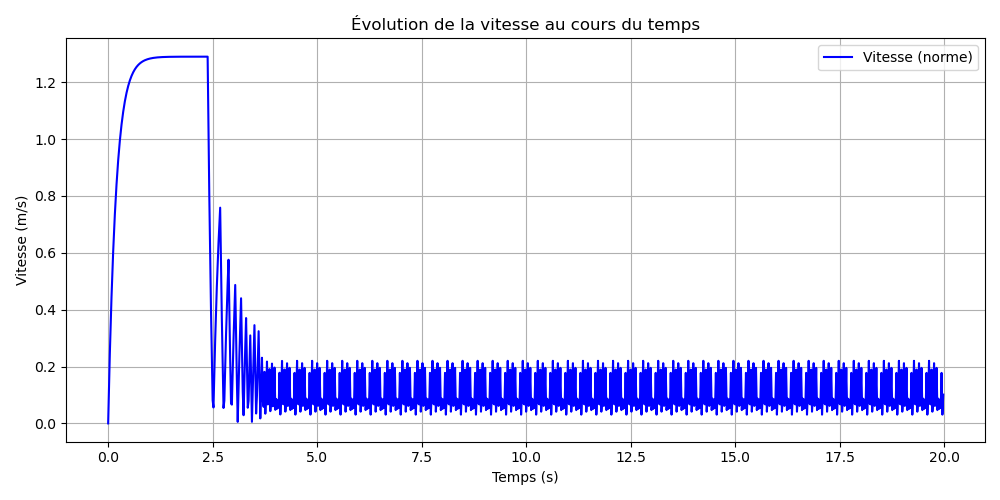
\includegraphics[width=\textwidth]{graph_vitesse.png} % moitié de la largeur du texte

Le résultat est bien cohérent on voit que la particule atteint à la manière d'une exponentielle inversé sa $v_{desiree}$ pour en suite l'atteindre totale. Dès que la position $(100,100)$ est atteinte sa vitesse décroit pour revenir vers la position. On voit qu'en suite la fonction devient périodique, la particule passe d'un bout à l'autre de la position (100,100) sans jamais l'atteindre.

\
\section{Explication du code}
\subsection{Structure et contextualisation}
\noindent Le code est divisé en trois modules distincts:
\begin{itemize}
	\item \textbf{main.py} s'occupe de dessiner la fênetre de gérer plusieurs actions il initialise le tableau de personne (tableau de particule)
	
	\item \textbf{physique.py} contient uniquement des fonction pour la gestion physique
\end{itemize}

\subsection{Modélisation physique}
\subsubsection{Force motrice}

Pour caculer la force motrice on applique simplement \eqref{eq:force_motrice}

\begin{minted}[frame=single, bgcolor=white, linenos]{python}
def force_motrice(personne):
    
    resultat = personne["vitesse_desiree"] * calcul_ei0(personne) 
    resultat -= personne["vitesse"]

    return  resultat /  personne["to"]
\end{minted}

La fonction \textbf{calcul\_i0} retourne le vecteur directionnel en soustrayant le point souhaité de la position actuelle de la personne, puis en normalisant le résultat.
\begin{minted}[frame=single, bgcolor=white, linenos]{python}
#position desiree
pt_souhaite = personne["destination"]
#direction 
vecteur_ei0 =  pt_souhaite - personne["position"]
vecteur_ei0 = [0, 1] if all(vecteur_ei0 == [0, 0]) else vecteur_ei0
# normalisation du vecteur
norm = np.linalg.norm(vecteur_ei0)
vecteur_ei0 = vecteur_ei0 / norm
\end{minted}

\subsubsection{Force social(s)}

Pour caculer on applique \eqref{eq:force_sociale}

\begin{minted}[frame=single, bgcolor=white, linenos, breaklines=true]{python}
def force_intercation_social(tab_personne, personne, indice, b0=config["b0"], seuil_interaction=50):

    for indice_personne, personne_autre in enumerate(tab_personne):
    		estTropLoin = 
        if indice_personne != indice and (np.linalg.norm(personne_autre["position"] - personne["position"]))  < seuil_interaction:

            a = personne["position"]
            b = personne_autre["position"]

            norme_ab = np.linalg.norm(a - b) - personne_autre["rayon"] - personne["rayon"]
			direction = (a - b) / np.linalg.norm(a - b)
			
            resultat = resultat + np.exp((- norme_ab / b0)) * direction

    return resultat
\end{minted}

La condition sert à ce qu'une particule n'agisse pas sur elle même, elle définie un seuil d'interaction pour réduire la compléxité temporelle ce qui est justifiable physiquement par le fait q'un personne trop n'agis pas sur nous (à partir d'un certain seuil).
\\
\\
Pour calculer $d_{ij}$ onprend la norme de la position de la personne avec la norme de la personne avec laquel elle intéragis on soustrait en suite les deux rayon qui correspond à $r_{ij}$. $\vec{n_{ij}}$ est le vecteur normal ( a - b ) qu'on norme pour avoir un vecteur unitaire. 


\subsubsection{Force répulsion mur}
La force de repulsion de mur est plus compliquée à calculer. Il faut la calculer pour chaque mur avec toujours un seuil d'intéraction (un mur agis sur nous que s'il nous touche). \textbf{$r_{ij}$} reste le même. Mais pour caculer \textbf{$d_{ij}$} cette fois ci on utilise pythagore.

\begin{minted}[frame=single, bgcolor=white, linenos, breaklines=true]{python}
def force_intercation_social_mur(personne, indice, b0 = config["b0"]):

    coord_a = np.array([50, 50])
    coord_b = np.array([600,50])
    coord_c = np.array([600,600])
    coord_d = np.array([50, 600])
    
    resultat = 0
    
    
    if not (personne["position"][1] > 310 and personne["position"][1] < 340) and personne["position"][0] < 600 - personne["rayon"]:
        mur_bc = distance_mur_vect(coord_b, coord_c, personne)
    
        resultat += np.exp(- mur_bc[0] / b0) * mur_bc[1]

    mur_ab = distance_mur_vect(coord_a, coord_b, personne)
    
    resultat += np.exp(- mur_ab[0] / b0) * mur_ab[1]

    mur_ad = distance_mur_vect(coord_a, coord_d, personne)

    
    resultat += np.exp(- mur_ad[0] / b0) * mur_ad[1] * -1

    mur_dc = distance_mur_vect(coord_d, coord_c, personne)

    resultat += np.exp(- mur_dc[0] / b0) * mur_dc[1] * -1

    return resultat
\end{minted}

\
La condition sert à ne pas agir si on a une porte.
\
La fonction \texttt{distance\_mur\_vect} utilise le théorème de Pythagore. Elle renvoie un tuple avec, premièrement, la distance entre le mur visé ($\mathbf{d_{ij}}$), ainsi que le vecteur normal ($\mathbf{n_{ij}}$). A PLUS DETAILLER +-*7g4rg


\subsubsection{Force interaction rectangle}

Pour cette méthode on a créé une fonction qui détermine le point le plus proche du rectangle.


\begin{minted}[frame=single, bgcolor=white, linenos, breaklines=true]{python}
def point_le_plus_proche_rectangle(personne : dict, rectangle : dict) -> np.array:
    # vecteur mur (un sommet) -> personne
    pers_mur = personne["position"] - np.array([rectangle["x"], rectangle["y"]])
    
    # le vecteur pour désigner la longeur du mur 
    # pourra dans le future, ne pas être aligner aux axes x y
    vecteur_mur1 = np.array([rectangle["longueur"], 0.])
    
    # le vecteur pour désigner la largeur du mur 
    vecteur_mur2 = np.array([0., rectangle["hauteur"]])
    
    # vérifie si personne n'est pas dans le mur
    est_pas_dans_mur = False
    
    
    k1 = np.dot(pers_mur, normalize(vecteur_mur1))
    if (k1 < 0.):
        k1 = 0.
        est_pas_dans_mur = True
    
    vecteur_mur1_longeur = np.linalg.norm(vecteur_mur1)
    if (k1 > vecteur_mur1_longeur):
        k1 = vecteur_mur1_longeur
        est_pas_dans_mur = True
    
    k2 = np.dot(pers_mur, normalize(vecteur_mur2))
    if (k2 < 0.):
        k2 = 0.
        est_pas_dans_mur = True
    
    vecteur_mur2_longeur = np.linalg.norm(vecteur_mur2)
    if (k2 > vecteur_mur2_longeur):
        k2 = vecteur_mur2_longeur
        est_pas_dans_mur = True
        
    return (
        np.array([rectangle["x"], rectangle["y"]])
      + k1 * (vecteur_mur1)/ vecteur_mur1_longeur
      + k2 * (vecteur_mur2)/ vecteur_mur2_longeur
    )

\end{minted}

\paragraph{Vecteurs de Projection :}

Soit un rectangle défini par ses coordonnées de coin inférieur gauche $(x, y)$, sa longueur $l$, et sa hauteur $h$. Nous définissons deux vecteurs :
\begin{itemize}
    \item $\vec{v}_{\text{longueur}} = (l, 0)$ : vecteur représentant la longueur du rectangle.
    \item $\vec{v}_{\text{hauteur}} = (0, h)$ : vecteur représentant la hauteur du rectangle.
\end{itemize}

\paragraph{Position Relative :}

La position de la personne par rapport au coin inférieur gauche du rectangle est donnée par le vecteur :
\[
\vec{p}_{\text{relatif}} = (x_{\text{personne}} - x, y_{\text{personne}} - y)
\]

\paragraph{Projection sur les Bords du Rectangle :}

Pour trouver le point le plus proche sur le rectangle, nous projetons $\vec{p}_{\text{relatif}}$ sur les vecteurs $\vec{v}_{\text{longueur}}$ et $\vec{v}_{\text{hauteur}}$. Les projections sont calculées comme suit :

\begin{align*}
k_1 &= \frac{\vec{p}_{\text{relatif}} \cdot \vec{v}_{\text{longueur}}}{\|\vec{v}_{\text{longueur}}\|^2} \\
k_2 &= \frac{\vec{p}_{\text{relatif}} \cdot \vec{v}_{\text{hauteur}}}{\|\vec{v}_{\text{hauteur}}\|^2}
\end{align*}

\paragraph{Ajustement des Projections :}

Les valeurs de $k_1$ et $k_2$ sont ajustées pour s'assurer qu'elles se situent dans les limites du rectangle :
\begin{itemize}
    \item Si $k_1 < 0$, alors $k_1 = 0$.
    \item Si $k_1 > l$, alors $k_1 = l$.
    \item Si $k_2 < 0$, alors $k_2 = 0$.
    \item Si $k_2 > h$, alors $k_2 = h$.
\end{itemize}

\paragraph{Calcul du Point le Plus Proche :}

Le point le plus proche sur le rectangle est alors donné par :
\[
\vec{p}_{\text{proche}} = (x, y) + k_1 \cdot \frac{\vec{v}_{\text{longueur}}}{\|\vec{v}_{\text{longueur}}\|} + k_2 \cdot \frac{\vec{v}_{\text{hauteur}}}{\|\vec{v}_{\text{hauteur}}\|}
\]

\begin{minted}[frame=single, bgcolor=white, linenos, breaklines=true]{python}
def force_intercation_rectangle(personne, rectangle, b0=config["b0"]):
    point = point_le_plus_proche_rectangle(personne, rectangle)
    
    
    distance_mur = np.linalg.norm(point - personne["position"]) - personne["rayon"]

    return 15. * np.exp(- distance_mur / b0) * normalize(personne["position"] - point)
\end{minted}

Pour finir on applique \eqref{eq:force_sociale} ici $r_{ij}$ = $r_i$ - 0 car pas de rayon.

\subsection{Resolution}

\textbf{Situation 1}

Bdf trois forces:
\begin{itemize}
	\item \textbf{forces motrices} \eqref{eq:force_motrice}
	\item \textbf{forces interactions personnes} \eqref{eq:force_sociale}
	\item \textbf{forces interactions murs} \eqref{eq:force_sociale}
\end{itemize}
Mais on peut ajouter aussi, les forces d'interaction avec les rectangle comme il n'y a pas de mur le vecteur sera $\vec{0}$.
\\
\\
\textbf{donc au final on obtient une fonction euler qui généralise les deux cas}
\\
\\
On revient à l'equa dif: \eqref{eq:eq_diff}, en utilisant euler 
\begin{minted}[frame=single, bgcolor=white, linenos, breaklines=true]{python}
def euler(tab_personne, personne,indice,obstacles, step=.02):
    """
        pb physique 
    """

    #cacul de la force motrice
    f_m = force_motrice(personne)

    #force des murs de la simulation
    f_m += force_intercation_social_mur(personne , indice)

    #force interaction personnes
    f_m += force_intercation_social(tab_personne, personne, indice)

    #forces obstacles
    f_m += force_interaction_obstacle(personne, obstacles)

    #projection sur Ux et Uy
    vitesse_x =  personne["vitesse"][0] + step * f_m[0]
    vitesse_y = personne["vitesse"][1] + step * f_m[1]

    #on actualise la position
    personne["position"] = np.array( [
        personne["position"][0] + vitesse_x,
        personne["position"][1] + vitesse_y 
    ])

    # v(t_n+&)
    personne["vitesse"] = np.array([
        vitesse_x,
        vitesse_y
    ])
\end{minted}

\section{Analyse}
\subsection{Situation 1}



\subsection{Situation 2}

\newpage



\section{Bibliographie}

Voici la liste:

\vspace{1em}

\begin{itemize}
	\item \href{https://journals.aps.org/pre/abstract/10.1103/PhysRevE.51.4282}{Social force model for pedestrian dynamics (Dirk Helbing et Péter Molnár)}
	\item \href{https://www.google.com}{Lien vers le dépo git}
	\item \href{https://www.wikipedia.org}{Wikipedia}
\end{itemize}

\end{document}

\end{document}


pdflatex -shell-escape index.tex



